%!TEX root = ../doc.tex
\documentclass[../doc.tex]{subfiles}

\begin{document}
\chapter{Introduction}
\Gls{trt} is a dominant mechanism of energy transfer in the high energy density regimes found in astrophysical phenomena and \gls{icf} experiments. 
Thermal radiation is emitted by all matter at a temperature greater than absolute zero. The human body, for example, emits radiation in the infrared region allowing our bodies to be visible on an infrared camera. In an ICF experiment, temperatures and pressures are high enough that thermal radiation is emitted in the ``soft X-ray'' region and is energetic and abundant enough to alter the pressure exerted on matter, impacting its motion.
This tightly coupled interplay between the motion of matter and thermal radiative heat transfer is characterized by the field of radiation-hydrodynamics \cite{castor2004radiation,mihalas1999foundations}. Here, we focus on the ``radiation'' part of radiation-hydrodynamics. 

Kinetic models of photon transport phenomena are regarded as first-principles models for \gls{trt}. These models are believed to be a key component in reducing the gap between simulation and experiment observed in \gls{hedp} experiments \cite{osti_1460933}.
Kinetic models are capable of capturing the physics that cheaper models (e.g.~radiation diffusion) miss but at the cost of orders of magnitude more computational work and memory usage. 
In fact, the kinetic TRT package used in radiation-hydrodynamics simulations of the \gls{nif} often occupies 90\% of the runtime and memory usage of the entire simulation. Algorithms that reduce the cost of modeling TRT can thus have a significant impact on the cost of the entire simulation, allowing scientists to perform faster design iterations and realize higher accuracy models for the same electricity bill. 
Existing codes are extremely optimized so reductions in time-to-solution must come from the development of novel algorithms. 

In this dissertation, numerical algorithms for efficiently solving the kinetic description of radiation's interaction with matter are developed, the aim being to design methods that can be readily extended and incorporated into the radiation-hydrodynamics codes used to model \gls{nif}. The algorithms are centered around the use of the radiation moment equations to accelerate the iterative solution of the kinetic equation. 
% The moment equations are closed using information from the kinetic equation so that, upon convergence, the moment system can reproduce the physics of the kinetic equation. 
Iterative acceleration is achieved through a bidirectional coupling: the kinetic equation \emph{informs} the moment system through closures while the moment system \emph{drives} the kinetic equation by computing the slow-to-converge physics \cite{CHACON201721}. Such algorithms are attractive in the context of radiation-hydrodynamics since the moment system can be directly coupled to the hydrodynamics equations providing separation between the expensive kinetic equation and the evolution of stiff multiphysics \cite{doi:10.13182/NSE16-45}. 

% The primary challenge in the development of these algorithms is the efficient numerical approximation of the moment system. The closures used to define the moment system often make the application of existing discretization techniques and efficient preconditioned iterative solvers difficult. 
% In addition, we target high-order discretization techniques in order to align with the methods in use for hydrodynamics simulations of \gls{nif}. The development of high-order discretizations for the moment system that can be efficiently solved with existing linear solver technology is the primary contribution presented in this dissertation. 

In this chapter, we further motivate the need for this research, provide an overview of the approach along with the gap in the literature this dissertation fills, discuss the objectives and scope of the research, and conclude with an outline of the content in this document. 

\section{Motivation}
\subsection{The National Ignition Facility}
\gls{nif} is a laser-based \gls{icf} research facility located at the \gls{llnl}. At the time of writing this dissertation, NIF houses the world's largest and most energetic laser consisting of 192 beam lines. The target bay of \gls{nif} is shown in Fig.~\ref{intro:nif} inside of which the 192 beam lines converge onto the interior surfaces of a dime-sized, cylindrical halhraum (depicted in Fig.~\ref{intro:halhraum}) positioned at the center of the target chamber. The laser heats the walls of the halhraum to extreme temperatures, creating an X-ray oven that bathes a BB-sized capsule of frozen hydrogen isotopes. The X-rays burn the fuel capsule initiating an ablation that compresses the hydrogen to densities and pressures comparable to those seen at the center of the sun. These conditions cause the hydrogen to fuse into helium and release tremendous energy. In August 2021, NIF was able to achieve a burning plasma where the fusion reaction was partially sustained by energy released by the fusion process \cite{Zylstra2022}. This achievement represents a 10x improvement over previous attempts and is an important step toward achieving ignition, where the energy released by the fusion reaction exceeds that of the laser energy used to seed the fusion reaction. 
% --- NIF pictures --- 
\begin{figure}
\centering
\begin{subfigure}{.49\textwidth}
	\centering
	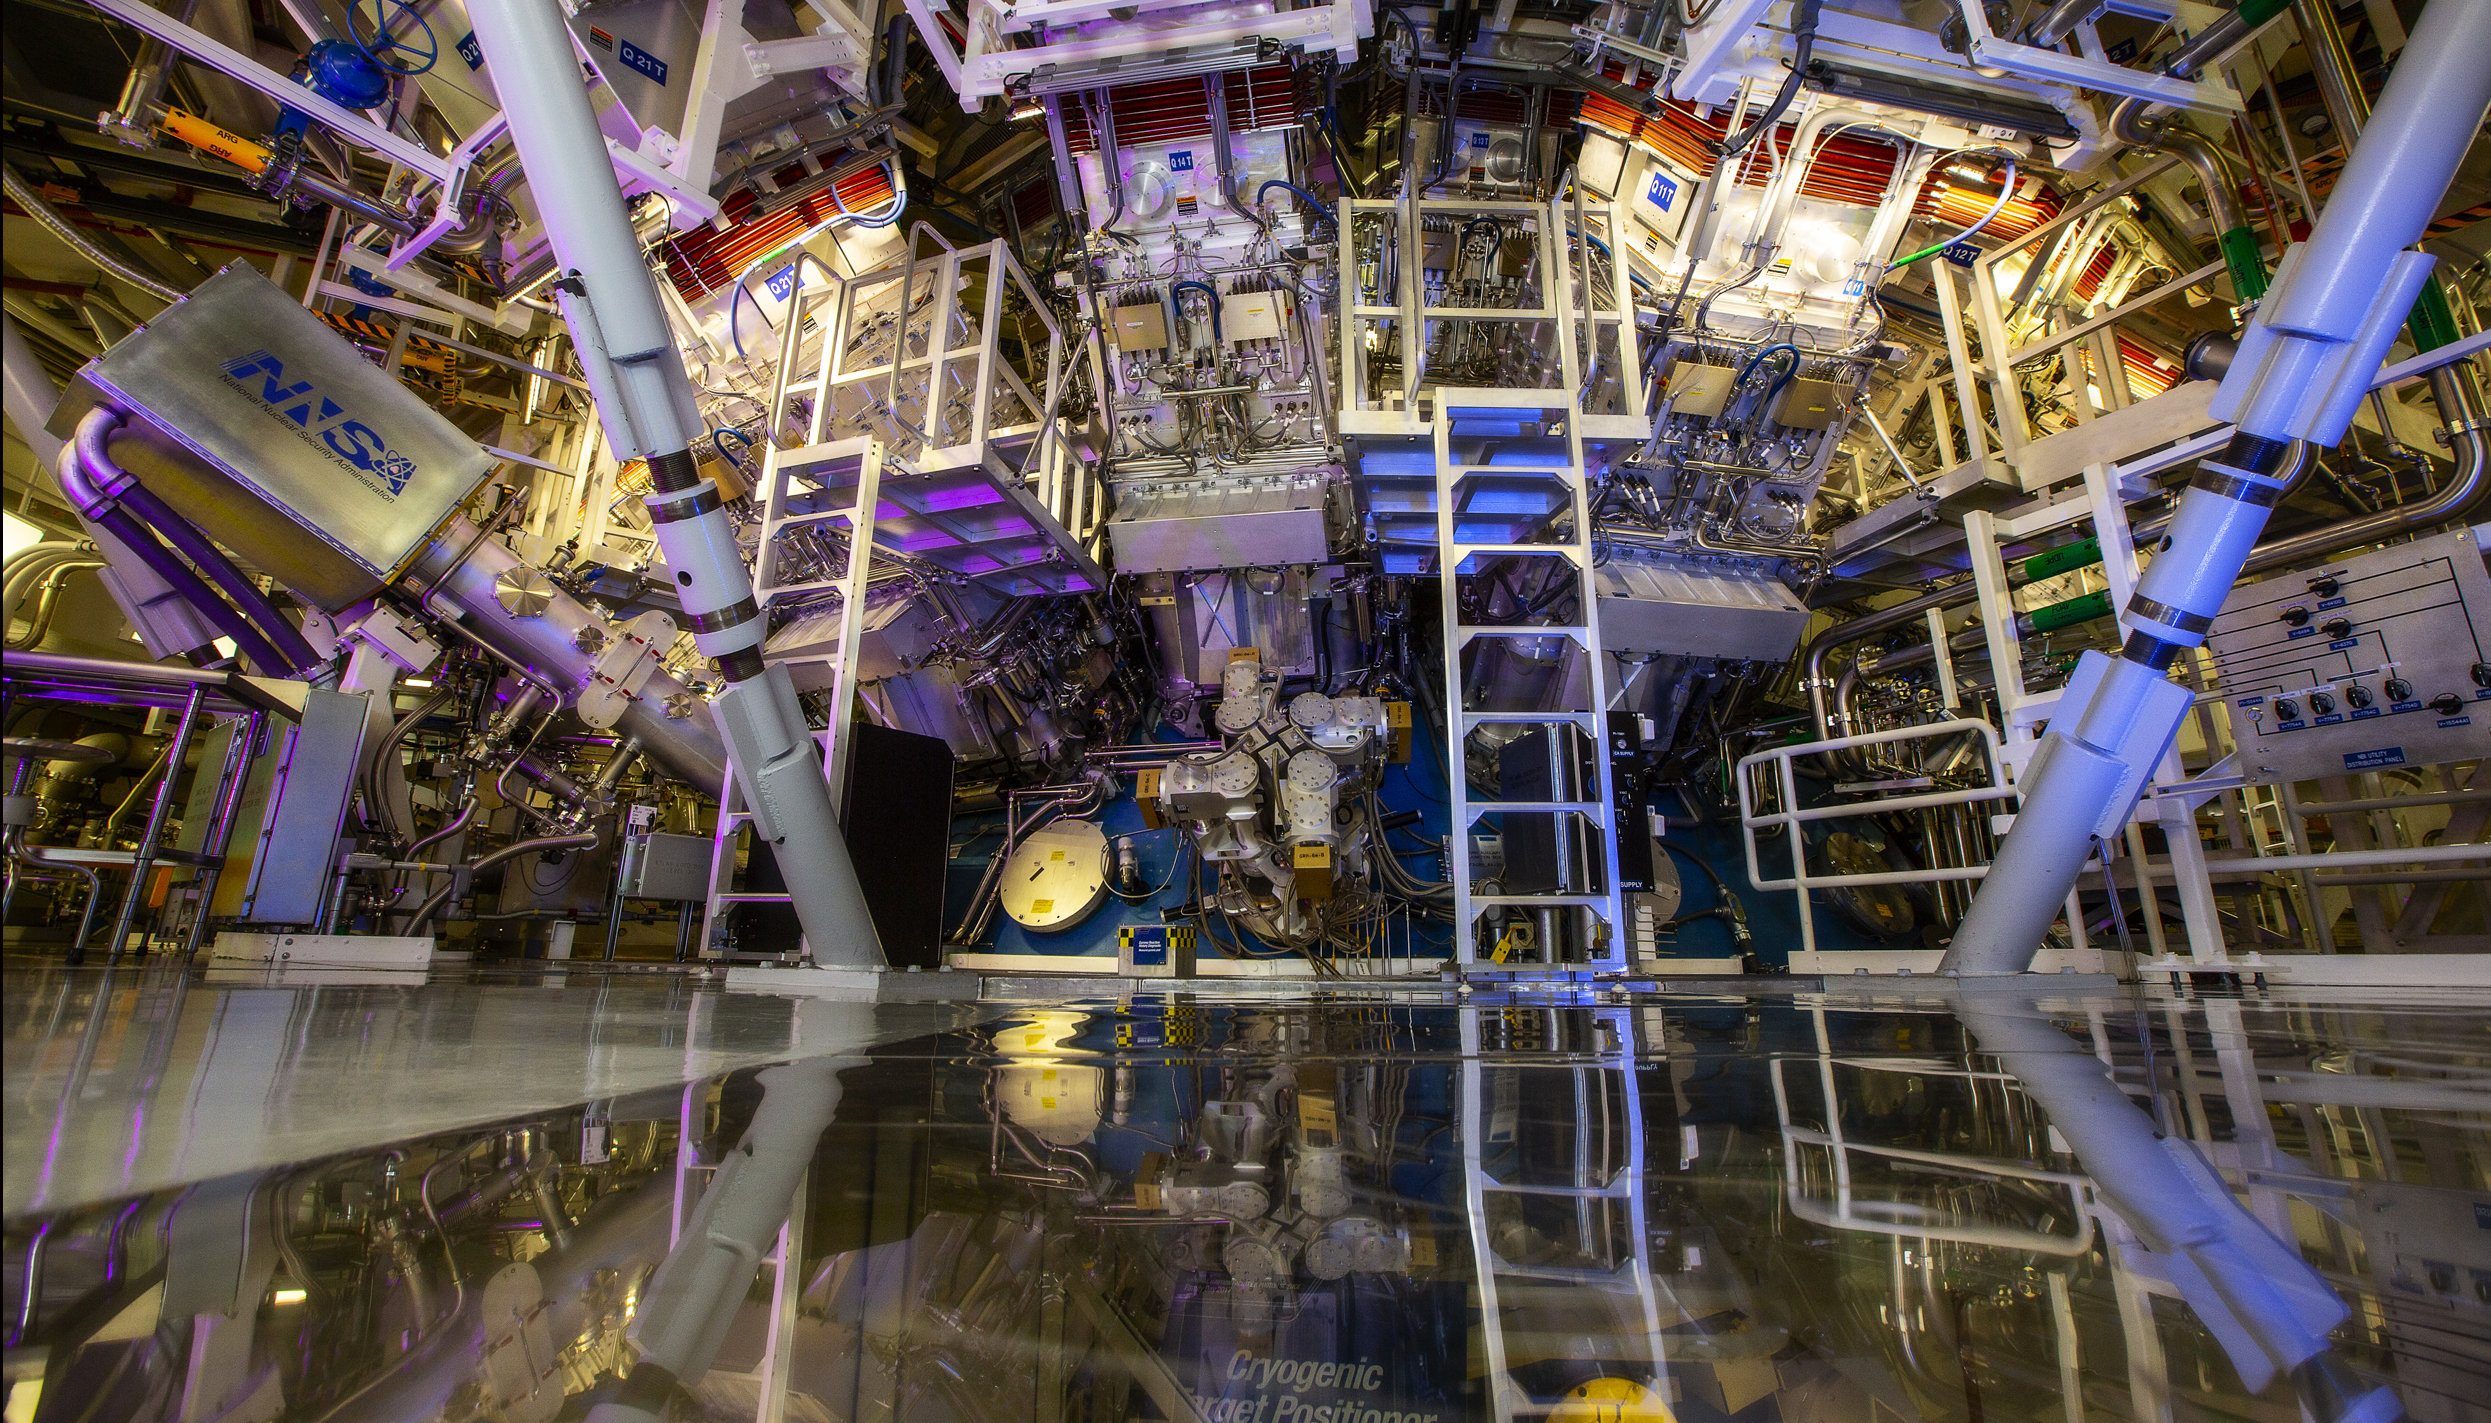
\includegraphics[height=1.75in]{data/img/nif.jpg}
	\caption{}
	\label{intro:nif}
\end{subfigure}
\begin{subfigure}{.49\textwidth}
	\centering
	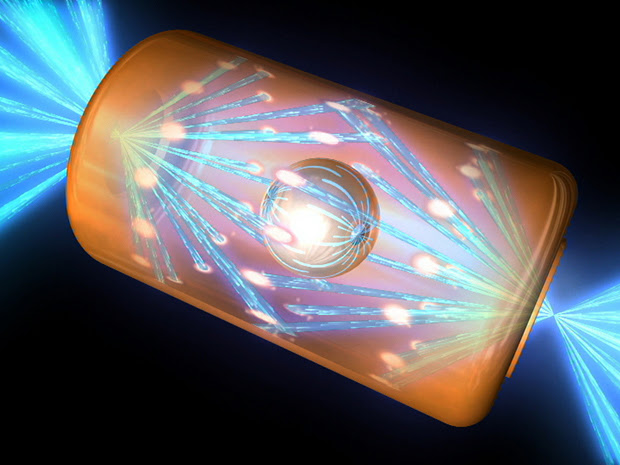
\includegraphics[height=1.75in]{data/img/halhraum.jpeg}
	\caption{}
	\label{intro:halhraum}
\end{subfigure}
\caption{(a) a photograph of the National Ignition Facility's target bay showing the laser entrance ports and diagnostics for measuring the properties of the experiment. (b) a depiction of the halhraum placed in the center of the target chamber shown in (a). The lasers impinge on the interior surface of the halhraum by entering through two openings on each side of the cylindrical halhraum. The walls of the halhraum heat to extreme temperatures, releasing X-rays that bathe the hydrogen fuel at the center of the halhraum. }
\end{figure}

The primary physical processes involved in a NIF experiment are: \gls{trt}, plasma physics, and nuclear reactions. Thermal radiation emitted by the walls of the halhraum is the primary driver of the ablation that initiates the fusion reaction. As the fuel heats, it also emits radiation which alters the distribution of energy and motion of the compression. The extreme temperatures and pressures present inside the halhraum mean matter exists in an ionized, plasma state where electrons are stripped free leaving a positively charged nucleus. This separation of charge induces electric and magnetic fields which greatly expand the range of possible motions and significantly complicate the study of the plasma's behavior \cite{chen2012introduction}. Finally, nuclear reactions are responsible for the production of fusion energy and the release of reaction byproducts, such as neutrons, that are an invaluable component for measuring the yield of a NIF experiment. 

The numerical simulation of these physical processes, along with many others, comprise a simulation suite that allows scientists to more efficiently design experiments and gain insight into the physics of \gls{icf} with reduced reliance on expensive and time-consuming physical experimentation. 
The demand for increasingly predictive models has made the numerical tools themselves topics of significant research spurring research investigations such as the one presented here in this dissertation.  

\subsection{Thermal Radiative Transfer}
The focus of this dissertation is the development of numerical methods for simulating the release and absorption of thermal radiation. We seek to model radiation as it moves through and interacts with a participating medium. 
Interactions of interest include matter absorbing and emitting radiation as well as scattering events where a photon's direction of travel and frequency are altered. 
% Fully describing radiation at a given point in time requires knowledge of where the radiation is in space, the direction it is traveling, and its frequency. 
The fundamental quantity of interest is the radiation's intensity, $I(\x,\Omegahat,\nu,t)$, which is a function of position, $\x$, direction of flight, $\Omegahat$, frequency, $\nu$, and time $t$. It represents the expected amount of energy per unit area, per unit solid angle, per unit frequency bandwidth, and per unit time. 
The seven-dimensional phase space is depicted in Fig.~\ref{intro:phase}. 
% --- phase diagram --- 
\begin{figure}
\centering
\includegraphics[width=.85\textwidth]{figs/phase.pdf}
\caption{A depiction of radiation transport's seven-dimensional phase space. }
\label{intro:phase}
\end{figure}
The intensity is mathematically described by the integro-partial differential equation known as the Boltzmann transport equation. 
Coupling the transport equation to a description of the conservation and exchange of energy between radiation and matter yields the equations of thermal radiative transfer. 

The emission of radiation is a highly nonlinear process with emissions scaling according to the fourth power of the temperature of the material \cite{pomraning2005equations}. The probabilities of the occurrence of absorption and scattering events also often have nonlinear dependence on the material's temperature. 
In addition, stimulated scattering, where the probability of scattering depends on the density of nearby radiation, leads to quadratic nonlinearities in the transport equation \cite{1986JQSRT..36..273K}. 
The above nonlinearities combined with the incredible expense associated with the transport equation's seven-dimensional phase space make the numerical simulation of \gls{trt} taxing on even the largest supercomputers. 

Numerical methods for solving the Boltzmann transport equation are classified into stochastic and deterministic methods. Stochastic methods use analog simulation to sample the movement of particles and their interactions. By sampling enough particles, the correct intensity can be found. Stochastic methods sample the solution's continuous dependence in angle and frequency and are thus considered the most accurate. 
However, they are very expensive due to the slow elimination of stochastic error.
Deterministic methods discretize each variable of the seven-dimensional phase space producing a large system of algebraic equations that must be solved efficiently. In practice, deterministic methods use iterative solution methods to solve the resulting algebraic system in order to avoid the memory cost associated with storing a system of equations corresponding to the entire phase space. In addition, well-designed iterative methods can significantly reduce the computational cost of solving the discrete transport equations. However, the design of such methods is a highly non-trivial task and has been the focus of significant research tracing back to the 1960s \cite{AL}. 

In this dissertation, we focus on deterministic methods and in particular those that employ the \gls{sn} angular model. In this approach, the transport equation is collocated at a discrete set of directions and integrations over the angular variable are approximated with a suitable quadrature rule. 
While a stochastic method such as \gls{imc} \cite{2001JCoPh.172..543G} has undoubtedly better better angular and frequency resolution (when stochastic variance is sufficiently reduced), it is typically infeasible to perform more than one nonlinear absorption-emission iteration per time step. In addition, \gls{imc} often struggles to preserve the diffusion limit when strong material discontinuities are present. Despite the known drawbacks of discrete frequency groups and ray effects, \gls{sn} methods are the de facto choice for kinetic models of \gls{trt} in \gls{hedp} simulations as they are computationally tractable enough to fully converge the nonlinear iteration at each time step, provide the solution in the entire phase space, preserve the diffusion limit, and can achieve iterative efficiency independent of the material parameters. This allows \gls{sn} methods to be both faster and more accurate than \gls{imc} in many problems of interest. 

In the context of radiation-hydrodynamics simulations, numerical models of \gls{trt} are used to compute the energy and momentum deposition of the radiation field onto the matter it is interacting with. In this case, we are interested in the amount of energy and momentum imparted to the material due to radiation traveling in all directions and with any frequency. In other words, radiation's effect on matter is communicated through integrals of the intensity over the direction and frequency variables. The resulting integrated quantities of the intensity are known as the moments. The fact that radiation and matter couple through a limited number of moments makes moment methods a natural choice for radiation-hydrodynamics simulations. 

\subsection{High-Order Finite Elements and Curved Meshes}
Recent trends in computer architecture, namely the ending of Moore's Law\footnote{the empirical observation that the number of transistors in an integrated circuit doubles every two years.}, indicate computers will be increasingly parallel and dependent on domain specific architectures such as \glspl{gpu}. This is especially evident in the Top500 list\footnote{\url{https://www.top500.org/}: a ranked list of the world's 500 most powerful supercomputers.}: from November 2011 to November 2021, the average number of CPU cores per socket rose from 6 to 27. 
In that same time span, the number of heterogeneous architectures increased from 39 to 150. 
Furthermore, it has been observed that floating point throughput is improving faster than memory latency and bandwidth. Thus, data movement will become increasingly expensive relative to computation. For GPU-accelerated computers, data movement is further compounded by the need to transfer data to and from the GPU. 

In light of these trends, the Department of Energy's Center for Efficient Exascale Discretizations (CEED) within the Exascale Computing Project (ECP) has targeted high-order finite element methods as one of it's main research thrusts. Compared to low-order methods, high-order methods are more accurate for the same number of unknowns (on smooth problems) and have better data reuse and locality. In other words, high-order methods have a higher floating point operation to memory access ratio\footnote{this ratio is called the \emph{arithmetic intensity}.} that makes them more amenable to efficient implementation on emerging \gls{hpc} architectures. 

In particular, the next-generation radiation-hydrodynamics code for modeling \gls{nif} at \gls{llnl} is based around the use of high-order finite elements on high-order (curved) meshes. In hydrodynamics simulations, high-order methods that use curved meshes have been shown to provide greater robustness (especially in the presence of significant mesh distortions), symmetry preservation, and strong scaling when compared to low-order methods \cite{blast,blast2,blast3}. In this framework, the material's velocity is represented with continuous finite elements and the thermodynamic variables are represented with discontinuous finite elements. This approach ensures the interfaces in the mesh remain continuous while allowing thermodynamic conservation to hold locally on each element. 
Figure \ref{intro:3p_anim} shows the evolution of the mesh associated with a third-order Lagrangian hydrodynamics simulation known as the ``triple point problem.'' In Lagrangian simulations, the mesh moves with the materials in order to preserve material interfaces exactly. Thus, as the materials deform, so does the mesh, leading to the deformed curved interfaces seen in the final mesh of Fig.~\ref{intro:3p_anim}. 
% --- triple point problem --- 
\begin{figure}
\centering
\foreach \f in {0,40,120,156}{
	\begin{subfigure}{.49\textwidth}
		\centering
		\includegraphics[width=\textwidth]{data/img/3p_anim/triple-\f.png}
		\caption{}
	\end{subfigure}
}
\caption{Selected time steps of the triple point problem. A third-order finite element representation is used to describe the mesh. A Lagrangian hydrodynamics approach is used where the mesh deforms with the materials in order to preserve material interfaces. This leads to the severely distorted curved elements depicted at the final time step. It is on such a mesh that we would like to solve radiation transport. Images taken from \url{https://computing.llnl.gov/projects/blast/triple-point-shock-interaction}.}
\label{intro:3p_anim}
\end{figure}

Coupling TRT to high-order hydrodynamics requires a transport method that is in some sense compatible with curved meshes. One possibility is to leverage existing transport methods by approximating the high-order mesh by refining it and using straight-edged elements. This approach, referred to as the low-order refined approach, is depicted for an example quadratic quadrilateral element in Fig.~\ref{intro:lor}. Note that this approach necessarily increases the number of unknowns, depicted as the nodes in each element, in the problem. 
\textcite{graph_sweeps} showed that realistic meshes generated from a high-order Lagrangian hydrodynamics code required a significant number of refinements to avoid simulation failure arising from inverted elements. In the context of the already memory and computation intensive seven-dimensional transport problem, this option can be impractical.   
In addition, under severe mesh distortions the low-order refined approach may not always produce an admissible mesh. 
Figure \ref{intro:lor_dist} shows an example of a distorted third-order element where the low-order refined process leads to an ill-defined mesh containing inverted and overlapping elements as well as elements with poor aspect ratios. In such case, a method that solves on the high-order mesh could continue whereas a method reliant on the low-order refined mesh would cause the simulation to fail. 
% --- low order refined simple --- 
\begin{figure}
\centering
\foreach \f in {lor.pdf,lor_1.pdf,lor4_1.pdf}{
	\begin{subfigure}{.32\textwidth}
		\centering
		\includegraphics[width=\textwidth]{figs/\f}
		\caption{}
	\end{subfigure}	
}
\caption{Depictions of the low-order refined process. (a) shows a quadratic quadrilateral element that has four unknowns. (b) and (c) show linear approximations to the geometry of the element in (a) that use one and two refinements, respectively. In order for the curved surfaces to be accurately captured, refinements are required. However, this necessarily increases the number of unknowns which can be impractical in the context of the already memory intensive radiation transport solve. }
\label{intro:lor}
\end{figure}
% --- low order refined impractical --- 
\begin{figure}
\centering
\foreach \f in {lor_dist.pdf,lor_dist_1.pdf,lor_dist4_1.pdf}{
	\begin{subfigure}{.32\textwidth}
		\centering
		\includegraphics[width=\textwidth]{figs/\f}
		\caption{}
	\end{subfigure}	
}
\caption{Depictions of the low-order refined process on a very distorted, cubic element. In this case, refining the high-order geometry shown in (a) leads to elements with poor aspect ratios, inverted elements, and elements that overlap. This is an example where naively refining the element would lead to simulation failure and is a motivating example for the need to solve on the high-order mesh.}
\label{intro:lor_dist}
\end{figure}

Radiation transport methods compatible with curved meshes are desired in order to avoid the necessary increase in unknowns and reduced robustness associated with the low-order refined approach. It is also possible that high-order methods could be beneficial in terms of accuracy and multiphysics compatibility with high-order hydrodynamics. However, these claims of increased accuracy and compatibility have yet to be demonstrated in large-scale, tightly coupled simulations. Discontinuous finite element representations of the energy density (scalar flux in nuclear engineering terminology) are preferred in order to have immediate multiphysics compatibility with the framework of \cite{blast}. High-order discontinuous finite element methods for radiation transport have received attention recently with the development of \gls{dg} discretizations of the \gls{sn} transport equations compatible with curved meshes in \cite{graph_sweeps,woods_thesis} and corresponding \gls{dsa} methods in \cite{ldrd_dsa,doi:10.1080/00295639.2020.1799603}. 
% However, high-order discretizations of the VEF equations compatible with curved meshes have not yet been developed. 
However, high-order moment-based transport algorithms compatible with curved meshes have not yet been developed. 

\section{Moment Methods for Radiation Transport}
Moment methods are a class of iterative schemes for solving kinetic equations. Example applications include radiation transport \cite{goldin}, plasma physics \cite{MASON1981233}, and ocean modeling \cite{10.1016/j.procs.2015.05.477}. \textcite{CHACON201721} provides an excellent survey of their 60 year history. These methods are characterized by iteratively coupling the kinetic equation to its statistical moments. 
Closures of the moment system are used such that, upon iterative convergence, the moment system is capable of reproducing the physics of the kinetic equation. 
In the case of radiation transport, the closures are weak functions of the solution, allowing the design of efficient and robust iterative schemes. 

In the radiation transport literature, moment methods have been shown to allow significant algorithmic flexibility in that any valid discretization of the moment system will yield a rapidly converging algorithm \cite{two-level-independent-warsa}. 
This is in stark contrast to preconditioning schemes, such as \gls{dsa}, which place severe restrictions on the discretization of the moment system in order to guarantee iterative efficiency \cite{A}. In the case where the transport and moment discretizations are not algebraically consistent, referred to as an ``independent'' moment method \cite{doi:10.1080/00411459308203810,two-level-independent-warsa}, the discrete moment and transport solutions will differ on the order of the spatial discretization error. Thus, the two solutions will be equivalent only in the limit as the mesh is refined. However, even in an under-resolved problem, moment methods still produce a ``transport solution'' in that the moment algorithm produces a discrete solution to an equivalent reformulation of the transport equation. Furthermore, moment methods generally preserve the thick diffusion limit \cite{diflim} and have conservation even if the transport discretization in isolation does not. Such properties are particularly useful in the context of multiphysics calculations since the lower-dimensional moment system can be directly coupled to the other physics components in place of the high-dimensional transport equation. Most importantly, moment methods allow the transport and moment discretizations to be chosen independently meaning each can be designed to be in some sense optimal for their intended use. 

In this section, we introduce the two classes of moment methods investigated in this dissertation. Relevant literature is discussed in order to identify the research gaps this dissertation fills. 

\subsection{The Variable Eddington Factor Method}
The \gls{vef} method \cite{mihalas,auer_vef}, also known as \gls{qd} \cite{goldin}, is a particular class of moment method that employs multiplicative closures. 
The closures are built from transport-dependent functionals that are bounded and possess small functional derivatives with respect to the transport solution. This allows the design of robust and efficient iterative schemes but comes with the costs of the moment system no longer being self-adjoint and, due to the nature of multiplicative closures, the resulting iteration being nonlinear. 
VEF has been applied to a wide range of transport and multiphysics problems including (but not limited to) nuclear reactor eigenvalue problems \cite{airstova_eigenvalue}, nuclear reactor kinetics \cite{doi:10.13182/NSE13-42}, and \gls{trt} \cite{anistratov1996nonlinear}. In addition, VEF performs well in problems having both optically thick and thin regions and treats anisotropic scattering equally well \cite{anistratov_fvm,ARISTOVA2000139}. 

VEF-based moment algorithms have been designed to improve efficiency in relation to all seven dimensions of the transport equation. 
% time 
\textcite{GHASSEMI2020109315} showed that different order temporal discretizations can be applied to the transport and VEF equations. Ongoing work suggests that time-stepping stability and accuracy can be maintained when just one transport inversion is performed per time step \cite{yee_mc21}. \textcite{anistratov2021implicit} used data compression techniques to reduce storage costs in time-dependent calculations. In astrophysics, VEF is used to simplify the implementation of coupling TRT to hydrodynamics and to avoid the memory cost of solving the time-dependent transport equation \cite{Jiang_2012,GNEDIN2001437,GEHMEYR1994320}. 
% space 
\textcite{Davis_2012} used a short characteristics discretization of the transport equation. \textcite{me} and \textcite{LOU2019258} designed a spatial discretization of the VEF equations to increase multiphysics compatibility. This algorithm was used to form the basis of an efficient radiation-hydrodynamics method in \cite{LOU2021110393}. \textcite{YEE2020109696} showed that robust convergence is maintained even when positivity-preserving methods are used inside the iteration. 
% energy
\textcite{anistratov2020nonlinear} solved the multigroup TRT equations by using a VEF method with multiple levels in frequency. The stability of this algorithm was analyzed in \cite{ANISTRATOV2019186}. It is also well-known that the multigroup eigenvalue problem can be solved with only the need for eigenvalue iterations on the one-group VEF equations \cite{AL}. 

The above techniques rely on the efficient solution of the discretized VEF moment equations. VEF methods reduce the overall cost of the simulation by trading inversions of the high-dimensional transport equation with inversions of the lower-dimensional VEF equations. In all of VEF's applications, the solution of the discretized VEF equations is buried under multiple nested loops corresponding to time integration, Newton iterations, eigenvalue iterations, multi-group iterations, and/or fixed-point iterations. The efficient iterative solution of the VEF equations is then crucial to the efficiency of the overall algorithm and is a prerequisite for the practicality of any VEF method. 

The unusual structure of the VEF equations and their lack of self-adjointness make the development of discretizations and their corresponding preconditioned iterative solvers difficult.
Previous work on discretizing the VEF equations includes finite volume \cite{anistratov_fvm,doi:10.1080/00411459308203810,QDBC,Jiang_2012,Jones2019TheQM}, finite difference \cite{WIESELQUIST2014343}, mixed finite element \cite{vallette,me,olivier_mandc,LOU2019258,LOU2021110393}, continuous finite element \cite{wieselquist,two-level-independent-warsa}, and discontinuous finite element \cite{dima_dfem} techniques. 
While considerable effort has been placed into the discretization of the VEF equations, to our knowledge, existing methods either rely on expensive and unscalable preconditioners such as block incomplete LU (BILU) factorization, cannot be solved with iteration counts independent of the mesh size, or do not mention solvers entirely. In addition, none of these methods are compatible with curved meshes or achieve higher than second-order accuracy in space. 

\textcite{two-level-independent-warsa} showed that VEF methods with and without algebraic consistency converged equivalently as long as the transport-dependent closures were properly represented. In particular, computing the VEF closures using finite element interpolation and \gls{sn} angular quadrature enabled rapid convergence for the independent discretizations they considered. 
Thus, an independent discretization of the VEF moment system has the potential to provide the rapid convergence of an algebraically consistent VEF method while enabling significant algorithmic flexibility. This flexibility can be used to define VEF methods that leverage existing linear solver technology and/or have increased multiphysics compatibility. 

\subsection{The Second Moment Method}
The \gls{smm} of Lewis and Miller \cite{lewis_miller} is another moment method designed for the radiation transport equation. Where VEF uses nonlinear, multiplicative closures to form the VEF moment system, the SMM moment system is formed using linear, additive closures. The original concept was to close the radiation diffusion system by means of transport-dependent corrections that vanish when the transport solution is a linear function in angle \cite{AL}. 
In this way, the SMM algorithm is able to form a transport method where the moment system is the symmetric radiation diffusion operator with additional transport-dependent source terms. This avoids the difficulty of developing discretizations and preconditioners for the non-symmetric VEF operator required by VEF methods and allows use of simpler iterative solvers such as the conjugate gradient method. 

A Fourier analysis of the iterative convergence of \gls{smm} was conducted by \textcite{cefus} where SMM was shown to have equivalent convergence as \gls{dsa}. It was also shown that VEF and SMM will converge equivalently when in close enough vicinity of the solution. Furthermore, they showed that SMM can be viewed as a VEF method that has been linearized about a linearly anisotropic solution. These results suggest the benefits of the VEF algorithm will extend to SMM. 

Since the SMM moment system is the simple radiation diffusion equation, discrete SMMs can leverage existing discretization and scalable solver technology immediately. However, the representation of the SMM correction sources shares many of the same discretization difficulties seen for the VEF moment system. Investigation into discrete SMMs is limited in the literature with the only previous work being \textcite{STEHLE2014325} and \textcite{https://doi.org/10.48550/arxiv.2102.09054}. \textcite{STEHLE2014325} developed a domain decomposition method where an SMM is used to couple transport and diffusion domains through interface conditions. The SMM moment system and correction sources were discretizated to be algebraically consistent with the upstream corner balance (UCB) \cite{ucb_maginot} \gls{sn} transport method. 
\textcite{https://doi.org/10.48550/arxiv.2102.09054} investigated a multilevel in energy algorithm for neutron transport problems. The discretization of the moment system was designed to be consistent with a lowest-order \gls{dg} discretization of the \gls{sn} transport equations. This method can be viewed as a linearization of the \gls{dg} VEF method from \cite{dima_dfem}. 
Neither of these methods attain higher than second-order accuracy or are compatible with curved meshes. Furthermore, independent SMMs have not yet been developed. 

\section{Objectives and Scope}
The goal of this work is to develop computationally efficient moment methods for solving the kinetic radiation transport equation that can be readily incorporated into the radiation-hydrodynamics codes used to model \gls{nif}. In particular, we seek to design discretizations for the moment system that have: 
	\begin{enumerate}
		\item high-order accuracy, 
		\item compatibility with curved meshes, and
		\item efficient preconditioned iterative solvers. 
	\end{enumerate}
These objectives are achieved using the independent approach. The flexibility of this approach allows use of any valid discretization of the moment equations as long as the closures are properly represented. Thus, we pursue the extension of discretization techniques developed for the model elliptic problem to the unusual structures of the VEF moment system and the SMM correction sources. Our hypothesis is that these discretization techniques and their associated preconditioned iterative solvers will also be effective for the VEF and SMM moment systems allowing the design of efficient moment methods. 

We limit the scope of this investigation to the steady-state, mono-energetic, linear Boltzmann equation with isotropic scattering. This simplified model is derived from the TRT system by neglecting time and frequency dependence and replacing the temperature coupling with isotropic scattering. This model problem emulates a single Newton iteration for each discrete frequency group in a full TRT simulation and thus represents a first step toward developing methods for the much more complicated TRT and radiation-hydrodynamics systems. The efficacy of this proxy problem has already been demonstrated as one of the methods presented in this dissertation has been successfully used in a frequency-independent TRT context \cite{yee_mc21}. 

\section{Outline}
The structure of this document is depicted graphically on page \pageref{preamble:interdependence}. 
We begin in Chapter \ref{chap:transport} with background on radiation transport. We present the equations of thermal radiative transfer and the simplifications that result in the steady-state Boltzmann equation that serves as our model problem. The chapter concludes with a derivation of the radiation diffusion approximation. 

Chapter \ref{chap:moment} derives the VEF and SMM moment systems by applying suitable closures to the angular moments of the model transport problem defined in Chapter \ref{chap:transport}. We present the techniques used in this document for solving the coupled transport-moment system and discuss the mathematical properties of the VEF and SMM closures, including their close connection through linearization. These properties are used to further motivate the need for the specialized discretization techniques developed here. 

Chapter \ref{chap:fem} provides an introduction to the finite element method. The key high-level ideas of weak forms and Sobolev spaces are motivated. We then define the finite element spaces used in subsequent chapters to discretize the transport equation and moment systems. These spaces are defined on a computational mesh and are built as piecewise polynomial functions on each element in the mesh. We provide implementation details on the representation of high-order meshes and the associated transformations needed to perform numerical integration over arbitrary elements. The chapter concludes with a brief description of preconditioned iterative solvers. 

The transport discretization used by both the VEF and SMM algorithms is defined in Chapter \ref{chap:sn}. We use the \gls{sn} angular model along with a \gls{dg} discretization in space. The efficient solution procedure known as the transport sweep is defined. Summaries of recent advances related to solving the \gls{sn} transport equations on high-order meshes are provided. This includes a graph algorithm to sweep on curved meshes with reentrant faces, discussion of numerically integrating the inflow conditions on curved faces, and the extension of positivity-preserving flux fixup methods to high-order solution representations. The chapter concludes with a discussion of the discrete moment algorithm. The closures for the moment system are computed using the \gls{sn} angular quadrature and finite element interpolation. We also present the construction of the transport equation's scattering source from the solution of the moment system. 

Chapters \ref{chap:dgvef}--\ref{chap:smm} contain the novel contributions of this dissertation. Discretizations of the moment system are presented that, when combined with the transport discretization from Chapter \ref{chap:sn}, lead to efficient high-order methods for solving the Boltzmann transport equation. Each chapter concludes with numerical results demonstrating the efficacy of the methods presented therein using the \gls{mms}, an asymptotic thick diffusion limit stress test problem on both an orthogonal and curved mesh, a multi-material proxy problem from \gls{trt} referred to as the crooked pipe problem, and a parallel weak scaling study of the preconditioned iterative solvers used to invert the moment systems. 

In Chapter \ref{chap:dgvef}, a \gls{dg} discretization is applied to the VEF moment system. We extend the unified analysis of DG methods for elliptic problems presented by \textcite{Arnold2002} to the VEF moment system to derive a family of discretizations for the second-order form of the VEF equations. This family of methods is efficiently preconditioned by the recently developed \gls{usc} preconditioner in \textcite{Pazner2021}. The DG framework is also used to derive a continuous finite element discretization of the VEF equations closely related to the method of \textcite{two-level-independent-warsa}. 

Chapter \ref{chap:rtvef} applies mixed finite element techniques to the VEF moment system. Such methods are chosen to match as closely as possible the methods used in the radiation diffusion package associated with the hydrodynamics code of \cite{blast}. We present three discretizations of which two can be effectively preconditioned using the standard techniques developed for the solution of mixed finite element discretizations of elliptic problems. 

Chapter \ref{chap:smm} shifts focus to SMM. The connection between SMM and VEF established in Chapter \ref{chap:moment} is leveraged to convert the discrete VEF algorithms developed in Chapters \ref{chap:dgvef} and \ref{chap:rtvef} to SMMs. This includes deriving \gls{dg}, continuous finite element, and mixed finite element-based SMMs. The resulting discrete moment systems are effectively preconditioned by their associated standard techniques on the simpler problem of radiation diffusion. 

Chapter \ref{chap:disc} serves two purposes. First, we use the DG VEF method to investigate generalities of the VEF method. This includes investigations into the effect of the choice of the initial guess for the preconditioned iterative solvers used to invert the moment systems and the use of Anderson acceleration to mitigate the slower convergence observed on meshes with reentrant faces. Second, we draw comparisons between all the methods presented in Chapters \ref{chap:dgvef}--\ref{chap:smm}. Performance on the common benchmarks of the thick diffusion limit, crooked pipe problem, and weak scaling are presented side-by-side in order to facilitate their comparison. 

Finally, Chapter \ref{chap:conclusions} summarizes the findings in this dissertation. Conclusions from each of Chapters \ref{chap:dgvef}--\ref{chap:disc} are presented. In addition, directions for future work concerning the extension of the methods presented here to a full radiation-hydrodynamics algorithm are included. 
\end{document}